% A LaTeX template for MSc Thesis submissions to 
% Politecnico di Milano (PoliMi) - School of Industrial and Information Engineering
%
% S. Bonetti, A. Gruttadauria, G. Mescolini, A. Zingaro
% e-mail: template-tesi-ingind@polimi.it
%
% Last Revision: October 2021
%
% Copyright 2021 Politecnico di Milano, Italy. NC-BY

\documentclass{Configuration_Files/PoliMi3i_thesis}

%------------------------------------------------------------------------------
%	REQUIRED PACKAGES AND  CONFIGURATIONS
%------------------------------------------------------------------------------

% CONFIGURATIONS
\usepackage{parskip} % For paragraph layout
\usepackage{setspace} % For using single or double spacing
\usepackage{emptypage} % To insert empty pages
\usepackage{multicol} % To write in multiple columns (executive summary)
\setlength\columnsep{15pt} % Column separation in executive summary
\setlength\parindent{0pt} % Indentation
\raggedbottom

% PACKAGES FOR TITLES
\usepackage{titlesec}
% \titlespacing{\section}{left spacing}{before spacing}{after spacing}
\titlespacing{\section}{0pt}{3.3ex}{2ex}
\titlespacing{\subsection}{0pt}{3.3ex}{1.65ex}
\titlespacing{\subsubsection}{0pt}{3.3ex}{1ex}
\usepackage{color}

% PACKAGES FOR LANGUAGE AND FONT
\usepackage[english]{babel} % The document is in English  
\usepackage[utf8]{inputenc} % UTF8 encoding
\usepackage[T1]{fontenc} % Font encoding
\usepackage[11pt]{moresize} % Big fonts

% PACKAGES FOR IMAGES
\usepackage{graphicx}
\usepackage{transparent} % Enables transparent images
\usepackage{eso-pic} % For the background picture on the title page
\usepackage{subfig} % Numbered and caption subfigures using \subfloat.
\usepackage{tikz} % A package for high-quality hand-made figures.
\usetikzlibrary{}
\graphicspath{{./Images/}} % Directory of the images
%\usepackage{caption} % Coloured captions
%\usepackage{xcolor} % Coloured captions
\usepackage{amsthm} % Coloured "Theorem"
\usepackage{thmtools}
\usepackage{xcolor}
\usepackage{float}

% STANDARD MATH PACKAGES
\usepackage{amsmath}
%\usepackage{amsthm}
\usepackage{amssymb}
\usepackage{amsfonts}
\usepackage{bm}
\usepackage[overload]{empheq} % For braced-style systems of equations.
\usepackage{fix-cm} % To override original LaTeX restrictions on sizes

% PACKAGES FOR TABLES
\usepackage{tabularx}
\usepackage{longtable} % Tables that can span several pages
\usepackage{colortbl}

% PACKAGES FOR ALGORITHMS (PSEUDO-CODE)
\usepackage{algorithm}
\usepackage{algorithmic}

% PACKAGES FOR REFERENCES & BIBLIOGRAPHY
\usepackage[
    colorlinks=true,
    linkcolor=black,
    anchorcolor=black,
    citecolor=black,
    filecolor=black,
    menucolor=black,
    runcolor=black,
    urlcolor=black
]{hyperref} % Adds clickable links at references
\usepackage{cleveref}
\usepackage[square, numbers, sort&compress]{natbib} % Square brackets, citing references with numbers, citations sorted by appearance in the text and compressed
\bibliographystyle{abbrvnat} % You may use a different style adapted to your field

% OTHER PACKAGES
\usepackage{pdfpages} % To include a pdf file
\usepackage{afterpage}
\usepackage{lipsum} % DUMMY PACKAGE
\usepackage{fancyhdr} % For the headers
\fancyhf{}

% Input of configuration file. Do not change config.tex file unless you really know what you are doing. 
% Define blue color typical of polimi
\definecolor{bluepoli}{cmyk}{0.4,0.1,0,0.4}

% Custom theorem environments
\declaretheoremstyle[
    headfont=\color{bluepoli}\normalfont\bfseries,
    bodyfont=\color{black}\normalfont\itshape,
]{colored}

% Set-up caption colors
\captionsetup[figure]{labelfont={color=bluepoli}} % Set colour of the captions
\captionsetup[table]{labelfont={color=bluepoli}} % Set colour of the captions
\captionsetup[algorithm]{labelfont={color=bluepoli}} % Set colour of the captions

\theoremstyle{colored}
\newtheorem{theorem}{Theorem}[chapter]
\newtheorem{proposition}{Proposition}[chapter]

% Enhances the features of the standard "table" and "tabular" environments.
\newcommand\T{\rule{0pt}{2.6ex}}
\newcommand\B{\rule[-1.2ex]{0pt}{0pt}}

% Pseudo-code algorithm descriptions.
\newcounter{algsubstate}
\renewcommand{\thealgsubstate}{\alph{algsubstate}}
\newenvironment{algsubstates}
{\setcounter{algsubstate}{0}%
\renewcommand{\STATE}{%
    \stepcounter{algsubstate}%
    \Statex {\small\thealgsubstate:}\space}}
{}

% New font size
\newcommand\numfontsize{\@setfontsize\Huge{200}{60}}

% Title format: chapter
\titleformat{\chapter}[hang]{
    \fontsize{50}{20}\selectfont\bfseries\filright}{\textcolor{bluepoli} \thechapter\hsp\hspace{2mm}\textcolor{bluepoli}{|   }\hsp}{0pt}{\huge\bfseries \textcolor{bluepoli}
}

% Title format: section
\titleformat{\section}
{\color{bluepoli}\normalfont\Large\bfseries}
{\color{bluepoli}\thesection.}{1em}{}

% Title format: subsection
\titleformat{\subsection}
{\color{bluepoli}\normalfont\large\bfseries}
{\color{bluepoli}\thesubsection.}{1em}{}

% Title format: subsubsection
\titleformat{\subsubsection}
{\color{bluepoli}\normalfont\large\bfseries}
{\color{bluepoli}\thesubsubsection.}{1em}{}

% Shortening for setting no horizontal-spacing
\newcommand{\hsp}{\hspace{0pt}}

\makeatletter
% Renewcommand: cleardoublepage including the background pic
\renewcommand*\cleardoublepage{%
    \clearpage\if@twoside\ifodd\c@page\else
    \null
    \AddToShipoutPicture*{\BackgroundPic}
    \thispagestyle{empty}%
    \newpage
    \if@twocolumn\hbox{}\newpage\fi\fi\fi}
\makeatother

%For correctly numbering algorithms
\numberwithin{algorithm}{chapter}

%----------------------------------------------------------------------------
%	NEW COMMANDS DEFINED
%----------------------------------------------------------------------------

% EXAMPLES OF NEW COMMANDS
%\newcommand{\bea}{\begin{eqnarray}} % Shortcut for equation arrays
%\newcommand{\eea}{\end{eqnarray}}
%\newcommand{\e}[1]{\times 10^{#1}}  % Powers of 10 notation

%----------------------------------------------------------------------------
%	ADD YOUR PACKAGES (be careful of package interaction)
%----------------------------------------------------------------------------

%----------------------------------------------------------------------------
%	ADD YOUR DEFINITIONS AND COMMANDS (be careful of existing commands)
%----------------------------------------------------------------------------

%----------------------------------------------------------------------------
%	BEGIN OF YOUR DOCUMENT
%----------------------------------------------------------------------------

\begin{document}
    \fancypagestyle{plain}{%
        \fancyhf{} % Clear all header and footer fields
        \fancyhead[RO,RE]{\thepage} %RO=right odd, RE=right even
        \renewcommand{\headrulewidth}{0pt}
        \renewcommand{\footrulewidth}{0pt}}

%----------------------------------------------------------------------------
%	TITLE PAGE
%----------------------------------------------------------------------------

    \pagestyle{empty} % No page numbers
    \frontmatter % Use roman page numbering style (i, ii, iii, iv...) for the preamble pages

    \puttitle{
        title=Software Engineering 2\\Requirements Analysis and\\Specification Document,
        name1=Irfan Cela - 10694934, % Author Name and Surname
        name2=Mario Cela - 10685242,
        name3=Alessandro Cogollo - 10571078,
%name4=Name Surname 4,
%name5=Name Surname 5,
        academicyear=2022-2023,
%groupnumber=GroupNumber
    } % These info will be put into your Title page

%----------------------------------------------------------------------------
%	PREAMBLE PAGES: ABSTRACT (inglese e italiano), EXECUTIVE SUMMARY
%----------------------------------------------------------------------------
    \startpreamble
    \setcounter{page}{1} % Set page counter to 1

%----------------------------------------------------------------------------
%	LIST OF CONTENTS/FIGURES/TABLES/SYMBOLS
%----------------------------------------------------------------------------

% TABLE OF CONTENTS
    \thispagestyle{empty}
    \tableofcontents % Table of contents
    \thispagestyle{empty}
    \cleardoublepage

%-------------------------------------------------------------------------
%	THESIS MAIN TEXT
%-------------------------------------------------------------------------
% In the main text of your thesis you can write the chapters in two different ways:
%
%(1) As presented in this template you can write:
%    \chapter{Title of the chapter}
%    *body of the chapter*
%
%(2) You can write your chapter in a separated .tex file and then include it in the main file with the following command:
%    \chapter{Title of the chapter}
%    \input{chapter_file.tex}
%
% Especially for long thesis, we recommend you the second option.

    \addtocontents{toc}{\vspace{2em}} % Add a gap in the Contents, for aesthetics
    \mainmatter % Begin numeric (1,2,3...) page numbering


    \chapter{Introduction}\label{ch:introduction}
    The EVs are eco-friendly vehicles that will be on our roads in the next future.
In order to keep global warming below 1.5°C, Europe have decided to reduce greenhouse gas emissions of CO2 per
person per year by 2030, and, by the same year, the IEA predicts that electric vehicles will have a market share
of roughly 30 percent, with a total number of 23 million e-cars on the roads.
EVs consumption is measured in kilowatt-hours per 100 kilometers, and most of the current electric cars can travel
between 150 and 350 kilometers on a single charge, but premium-brand models can currently cover more than 500
kilometers.

In this context, when people use an electric vehicle, knowing where to charge it and carefully planning the
charging process in such a way that it introduces minimal interference and constraints on our daily schedule
is of great importance.

That's were \verb|eMALL| operates: it can find charging stations owned by several Charging Point Operators - CPO - and,
considering the activities in user's schedule, it can propose the best possible path of charging process
in order to minimize the cost and the waisted time at the station.


\section{Purpose}
\label{sec:purpose}
\newcounter{g}
\setcounter{g}{1}
\newcommand{\cg}{\theg\stepcounter{g}}
\begin{table}[H]
    \centering
    \begin{tabular}{ |l|p{0.9\linewidth}| }
        \hline
        \textbf{ID} & \textbf{Description}                                                                                                     \\
        \hline
        G\cg        & The EVD can see charging stations nearby a specific location on the map                                                  \\
        \hline
        G\cg        & The EVD can get the detailed information of charging stations                                                            \\
        \hline
        G\cg        & The EVD can search for special offer provided by charging stations                                                       \\
        \hline
        G\cg        & The EVD can book a charge for his EV at a charging station for a specified time frame                                    \\
        \hline
        G\cg        & The EVD can pay for the recharging service                                                                               \\
        \hline
        G\cg        & Given the destination inserted in an activity in his calendar application, the EVD receives suggestions to charge his EV \\ %TODO: not correctly explained
        \hline
    \end{tabular}
    \caption{The goals.}
    \label{tab:goals_tab}
\end{table}


\section{Scope}
\label{sec:scope}
\newcounter{wp}
\setcounter{wp}{1}
\newcommand{\cwp}{\thewp\stepcounter{wp}}
\begin{table}[H]
    \begin{center}
        \begin{tabular}{ |l|p{0.8\linewidth}| }
            \hline
            \textbf{ID} & \textbf{Description}                                               \\
            \hline
            WP\cwp      & The DSO provides energy to charging stations                       \\
            \hline
            WP\cwp      & The EVD wants to charge his EV's battery                           \\
            \hline
            WP\cwp      & The EVD wants to know the prices of a specific charging station    \\
            \hline
            WP\cwp      & The EVD wants to know if there are any special offer he can redeem \\
            \hline
            WP\cwp      & The EVD wants to know the position of a specific charging station  \\
            \hline
            WP\cwp      & An eMSP actives a new offer for his customers                      \\
            \hline
            WP\cwp      & The CPO have deals with eMSP and offer them their charging station \\
            \hline
            WP\cwp      & The EVD pays for the service                                       \\
            \hline
            WP\cwp      & The EVD inserts a new activity in his calendar                     \\
            \hline
            WP\cwp      & Charging Points are distributed in the territory                   \\
            \hline
            WP\cwp      & CPO buys energy from a DSO at the price defined by the latter      \\
            \hline
            WP\cwp      & CPO defines the selling price of electricity                       \\
            \hline
            WP\cwp      & CPO defines special offers for its customers                       \\
            \hline
            WP\cwp      & The EVD connects the plug of the charging point to the EV          \\
            \hline
            WP\cwp      & The EV reaches the desired level of battery charge                 \\
            \hline
%TODO: evaluate the WP ``The EVD has a calendar where he inserts his activities'' with respect to WP8
%TODO: possibly a domain assumption ``The EV uses a GPS module for its localization''
%TODO: we have to insert as a domain assumption that our system is compatible only with EVs system navigation because
%            we never speak about phones, but only about EVs
%TODO: possibly a domain assumption ``The EV uses internet connection in order to communicate with CPMS' API''
%TODO: possibly a domain assumption ``Each EV has compatibility with a particular charging plug''
%TODO: possibly a domain assumption ``The EV's navigation system provides information about its GPS''
%TODO: possibly a domain assumption ``The EV's navigation system provides information about its average consumption''
%TODO: possibly a domain assumption ``The EV's navigation system provides information about its battery status''
%TODO: possibly a domain assumption ``The eMSP offers API in order to manage charging services''
%TODO: possibly a domain assumption ``The eMSP offers the availability of charging points in its charging stations through its API''
%TODO: possibly a domain assumption ``The eMSP provides charging station location information to eMSPs thanks to its API''
%TODO: possibly a domain assumption ``The eMSP shows to EVDs the ability to book charging stations up to a week in advance''
%TODO: possibly a requirement ``eMSP allows the EVD to be in place for the check up to 15 minutes from the booked time''
%TODO: possibly a domain assumption: The EVD has a payment service that allows him to pay digitally
%            It cannot be a WP because the eMSP is already part of the system, and furthermore is not exclusively part
%            of the reality and then not a WP.
        \end{tabular}
    \end{center}
    \caption{World Phenomenas.}
    \label{tab:worldph_tab}
\end{table}

\newcounter{sp}
\setcounter{sp}{1}
\newcommand{\csp} {\thesp\stepcounter{sp}}
\begin{center}
    \begin{longtable}{ |l|p{0.5\linewidth}|l|l| }
        \hline
        \textbf{ID} & \textbf{Description}                                                                                                      & \textbf{Controller} & \textbf{Observer} \\
        \hline
        SP\csp      & The EVD creates an account in the eMALL system                                                                            & EVD                 & eMALL             \\
        \hline
        SP\csp      & The EVD logs in eMALL                                                                                                     & EVD                 & eMALL             \\
        \hline
        SP\csp      & eMALL gets EVD's current position                                                                                         & eMALL               & EVD               \\
        \hline
        SP\csp      & The EVD asks for the list of charging stations nearby to his/her position to eMALL                                        & EVD                 & eMALL             \\
        \hline
        SP\csp      & eMALL returns the list of all the charging stations nearby his/her position to the EVD                                    & eMALL               & EVD               \\
        \hline
        SP\csp      & The EVD asks for detailed information about a specific charging station to eMALL                                          & EVD                 & eMALL             \\
        \hline
        SP\csp      & eMALL returns the charging cost per kWh of the charging station specified by the EVD                                      & eMALL               & EVD               \\
        \hline
        SP\csp      & eMALL returns the charging cost per minute of the charging station specified by the EVD                                   & eMALL               & EVD               \\
        \hline
        SP\csp      & eMALL returns the cost per minute of the additional fare for late unplugging of the charging station specified by the EVD & eMALL               & EVD               \\
        \hline
        SP\csp      & eMALL returns the charging power of the charging station specified by the EVD                                             & eMALL               & EVD               \\
        \hline
        SP\csp      & eMALL returns the types of connectors accepted by the charging points of the charging station specified by the EVD        & eMALL               & EVD               \\
        \hline
        SP\csp      & eMALL returns the number of charging points of the charging station specified by the EVD                                  & eMALL               & EVD               \\
        \hline
        SP\csp      & eMALL returns the current status (available, occupied, maintenance) of the charging station specified by the EVD          & eMALL               & EVD               \\
        \hline
        SP\csp      & The EVD asks for special offers that he/she can redeem to eMALL                                                           & EVD                 & eMALL             \\
        \hline
        SP\csp      & eMALL returns all the active special offers to the EVD                                                                    & eMALL               & EVD               \\
        \hline
        SP\csp      & The EVD asks for the schedule of a specific charging station to eMALL                                                     & EVD                 & eMALL             \\
        \hline
        SP\csp      & eMALL returns the schedule of the charging station specified by the EVD                                                   & eMALL               & EVD               \\
        \hline
        SP\csp      & The EVD specifies the timeframe he/she wants to be reserved for his booking                                               & EVD                 & eMALL             \\
        \hline
        SP\csp      & The EVD books a charging point for a specific plug through eMALL                                                          & EVD                 & eMALL             \\
        \hline
        SP\csp      & The EVD pays for a caution before booking a charging session through eMALL                                                 & EVD                 & eMALL            \\
        \hline
        SP\csp      & The EVD inserts a new payment method and the required information into eMALL                                              & EVD                 & eMALL             \\
        \hline
        SP\csp      & eMALL returns the outcome of the validity of the payment method inserted by the EVD                                       & eMALL               & EVD               \\
        \hline
        SP\csp      & The EVD asks to unlock the charging point he/she has booked to eMALL                                                      & EVD                 & eMALL             \\
        \hline
        SP\csp      & The EVD connect the EV to the charging point and starts the charging process                                              & EVD                 & eMALL             \\
        \hline
        SP\csp      & eMALL notifies the EVD of the current state of the charging process (battery's level, current cost, estimated time, ...)  & eMALL               & EVD               \\
        \hline
        SP\csp      & The EVD pauses the charging session                                                                                       & EVD                 & eMALL             \\
        \hline
        SP\csp      & The EVD ends the charging session                                                                                         & EVD                 & eMALL             \\
        \hline
        SP\csp      & eMALL notifies the EVD that the battery of his/her EV is charged                                                          & eMALL               & EVD               \\
        \hline
        SP\csp      & eMALL suggests the EVD to end the charging session after a defined level of the EV's battery is reached                   & eMALL               & EVD               \\
        \hline
        SP\csp      & The EVD pays for the charging session using the module offered by eMALL                                                   & EVD                 & eMALL             \\
        \hline
        SP\csp      & eMALL returns the outcome of the payment done by the EVD                                                                  & eMALL               & EVD               \\
        \hline
        SP\csp      & eMALL notifies the EVD about the need of charging the EV                                                                  & eMALL               & EVD               \\
        \hline
        SP\csp      & The CPO creates a Charging Point Operator account on eMALL                                                                & CPO                 & eMALL             \\
        \hline
        SP\csp      & The CPO adds a new charging station in its profile specifying all the needed information                                  & CPO                 & eMALL             \\
        \hline
        SP\csp      & The CPO updates information of an existing charging station                                                               & CPO                 & eMALL             \\
        \hline
        SP\csp      & The CPO activates a new special offer for its charging stations                                                           & CPO                 & eMALL             \\
        \hline
        SP\csp      & The CPO manually updates the DSO which provides it energy                                                                 & CPO                 & eMALL             \\
        \hline
        SP\csp      & The CPO updates the selling price of its electricity                                                                      & CPO                 & eMALL             \\
        \hline
        SP\csp      & The CPO sets the battery capacity of a charging station                                                                   & CPO                 & eMALL             \\
        \hline
        SP\csp      & The CPO asks for information about the DSOs to eMALL                                                                      & CPO                 & eMALL             \\
        \hline
        SP\csp      & eMALL returns the information about the DSOs to the CPO                                                                   & eMALL               & CPO               \\
        \hline
        SP\csp      & eMALL gets EVD's current schedule from his/her calendar                                                                   & eMALL               & EVD               \\
        \hline
        SP\csp      &                                                                                                                           &                     &                   \\
        \hline
        \caption{Shared Phenomenas.}
        \label{tab:sharedph_tab}
    \end{longtable}
\end{center}


\section{Definition, Acronyms, Abbreviations}
\label{sec:definition_acronyms_abbreviations}
\begin{table}[H]
    \begin{center}
        \begin{tabular}{ |l|l| }
            \hline
            \textbf{Acronyms} & \textbf{Definition}                              \\
            \hline
            eMSP              & e-Mobility Service Provider                      \\
            \hline
            CPO               & Charging Point Operator                          \\
            \hline
            CPMS              & Charge Point Management System                   \\
            \hline
            DSO               & Distribution System Operator                     \\
            \hline
            RASD              & Requirements Analysis and Specification Document \\
            \hline
            WP                & World Phenomena                                  \\
            \hline
            SP                & Shared Phenomena                                 \\
            \hline
            GX                & Goal Number X                                    \\
            \hline
            EVD               & Electric Vehicle Driver                          \\
            \hline
        \end{tabular}
        \caption{Acronyms used in the document.}
        \label{tab:acronyms}
    \end{center}
\end{table}


\section{Revision history}
\label{sec:revision_history}


\section{Reference Documents}
\label{sec:reference_documents}
The specification document \verb|Assignment RDD AY 2022-2023.pdf|.


\section{Document Structure}
\label{sec:document_structure}
The document is structured in six sections, as described below.

First section introduce the goals of the project, purposes, and a brief analysis on world and shared phenomena;
abbreviations and definitions useful to understand the problem are listed as well.

The following section, the second one, provides an overall description of the problem: here scenarios and further
details on domain, and scenarios are included, aside from more product and user characteristics, assumptions,
dependencies and constraints.

Later on, the third section focuses on the specific requirements and provides a more detailed analysis of external
interface requirements, functional requirements and performance requirements.

Lastly, the fourth section provides a formal analysis, using alloy.
This chapter is crucial to prove the correctness of the model described in the previous sections, and should focus on
reporting results of the checks performed and meaningful assertions.

Section five reports the effort spent by each group member in the redaction of this document, meanwhile the last
section simply lists bibliography references and other resources used to redact this document.



    \chapter{Overall Description}\label{ch:overall_description}
    \section{Product perspective}
\label{sec:product_perspective}%

\subsection{Class Diagrams}
\label{subsec:class_diagrams}%
The figure below lists and describes the classes involved in the system, their basic functionalities, their basic attributes,
and the relationships between them.
Some suggestions for a further expansion and deepening of the diagram below could be to evaluate the use of a decorator
pattern to implement the ``Fee'' class;
also, to evaluate the use of a status pattern to assign the state of a charging point (free, booked, occupied, broken).
Furthermore, another suggestion could be to adopt the factory pattern to implement the ``plug'' interface.
\begin{figure}[H]
    \begin{center}
        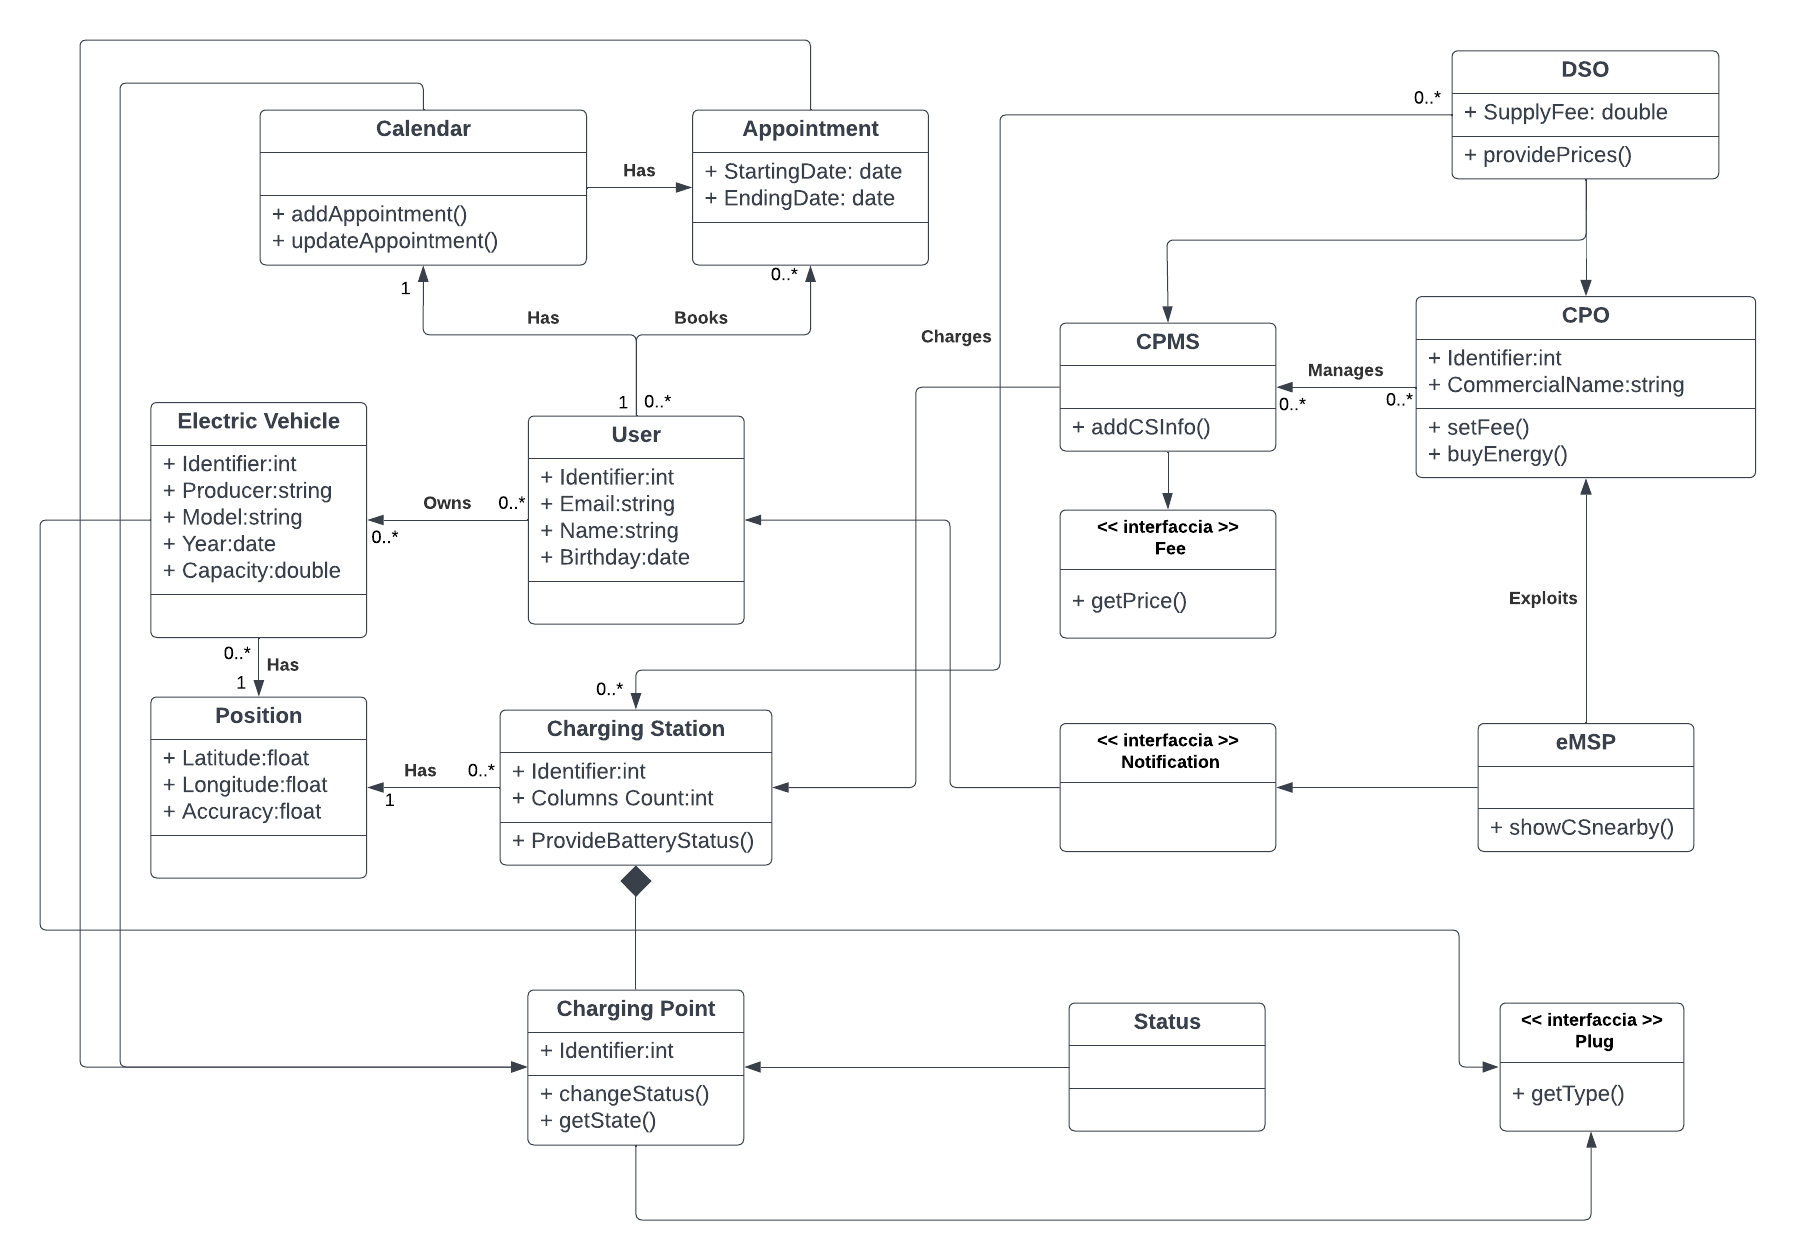
\includegraphics[width=0.9\linewidth]{ClassDiagrams/Class Diagram - noPatterns}
        \caption{A simplified Class Diagram}
        \label{fig:class_diagram}
    \end{center}
\end{figure}

\subsection{State Diagrams}
\label{subsec:state_diagrams}%

\paragraph{The EVD gets position and characteristics of charging stations at a certain location.}
EVD Andrew is going to use his car to go to the university for the Software Engineering 2 exam, but his EV is out of battery.
So, he needs to decide where to charge his vehicle.
To do that, he opens the \verb|eMALL| application and enters the map section.
At first, he sees if there is any charging station around him, but unfortunately at his current position,
there is only one charging station, which is shown as in maintenance.
So, he decides to see where to charge his EV nearby the university, inserting Milan in the location bar.
From the huge amount of charging stations, he decides to decide the one that costs less than the other ones.
So, he selects a charging station and gets its additional information.
He goes on searching other stations until he finds the best one for him.
At this point, the navigation process ends.

It is shown a state diagram that summaries the flow of activities done in the charging stations navigation process:
\begin{figure}[H]
    \begin{center}
        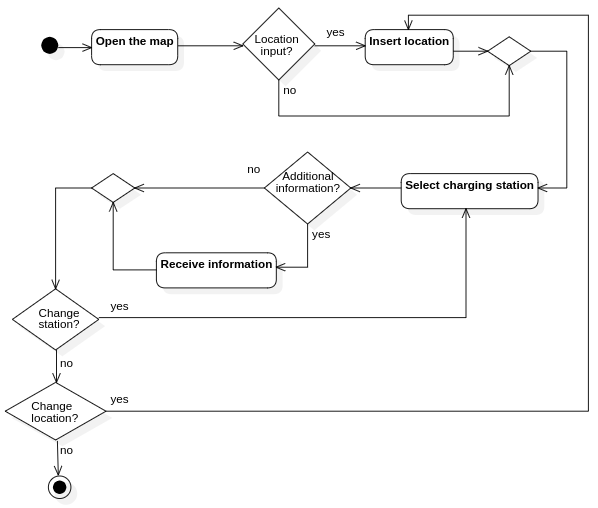
\includegraphics[width=0.8\linewidth]{StateDiagrams/get_charging_stations_location_state_diagram}
        \caption{Get locations of charging stations state diagram}
        \label{fig:locations_sd}
    \end{center}
\end{figure}

\paragraph{EVD books a charge at a specified charging station at a certain timeframe.}
Andrew needs to book a charge for his EV\@.
He selects a charging station on the map and enters the booking section.
If the charging station cannot offer a reservation to EVD because of no availability status, it alerts the EVD\@.
Andrew has to decide in which timeframe he wants the charging point to be reserved.
So, he gets the availability schedule of the charging station and selects when he thinks to go to charge.
The system asks to pay a deposit to the EVD, which makes the payment.
Finally, the EVD receives an e-mail with all the information that confirms the reservation.

It is shown a state diagram that summaries the activities in the booking process:
\begin{figure}[H]
    \begin{center}
        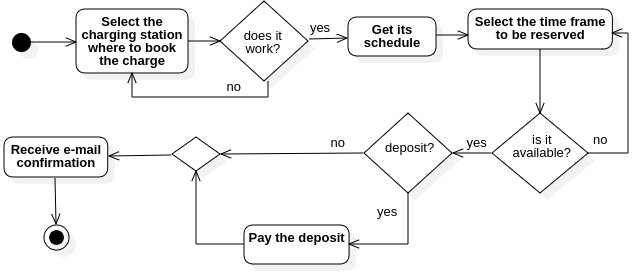
\includegraphics[width=0.9\linewidth]{StateDiagrams/book_a_charge_state_diagram}
        \caption{Book a charge state diagram}
        \label{fig:booking_sd}
    \end{center}
\end{figure}

\paragraph{CPO adds charging points in its CPMS.}
\verb|SOLARIS| is the new company of the successful businessman Hugh Peter.
They decided to trust the \verb|eMALL| project, entrusting them with the responsibility of managing their IT infrastructure.
After logging in, they start inserting new charging points owned by them and distributed throughout the territory.
If it belongs to a new charging station, he needs to create it too.
So, they insert all the requested information (location, costs, connectors, power, etc.).
After they confirm and submit what they inserted, they can add a new charging point.
Otherwise, the process ends.

It is shown a state diagram to summaries the activities in the charging points insertion process:
\begin{figure}[H]
    \begin{center}
        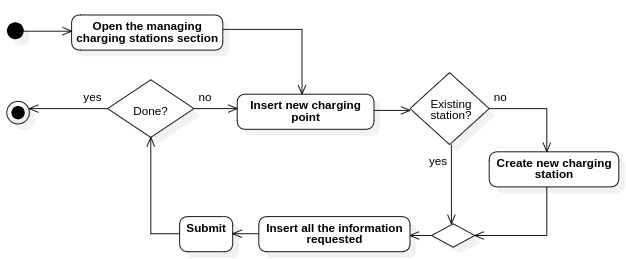
\includegraphics[width=0.9\linewidth]{StateDiagrams/insert_charging_points_state_diagram}
        \caption{Insert charging points state diagram}
        \label{fig:insert_charging_points_sd}
    \end{center}
\end{figure}

\subsection{Scenarios}
\label{subsec:scenarios}%

\paragraph{Unregistered EVD creates an account.}
Mike Hoar has his EV and is looking for an application that offers the chance to charge his vehicle and smartly plan a charging process depending on the battery status and his daily schedule.
Fortunately, he finds out \verb|eMALL|\@.
So, he immediately proceeds to create an account.
At first, he opens the application and goes to the ``sign up'' section.
He inserts his name, second name, date of birth, living address, e-mail address, password, and telephone number.
He receives an e-mail with a 6-digit code to be inserted in the new window shown by the \verb|eMALL| system to confirm his e-mail address.
After accepting the terms \& conditions and submitting all the inserted information, the system creates his account, and he can start using the application.

\paragraph{The EVD charges his/her EV.}
After booking a charge, NomeFantasia goes to the charging station at the chosen hour.
After turning off the EV, he opens the \verb|eMALL| application and enters the charge section.
From the set of close charging points, he selects which one has the serial number he received by \verb|eMALL| by e-mail
when he booked the charge.
So, he asks to charge the EV at that charging point.
After verifying that the EVD can charge at that charging point, the application communicates to the user that the
connectors are now unlocked and ready for charging his EV\@.
While the EV is in charge, the system notifies the EVD of the current status of the charging process.
When the process ends, he unplugs the connector, pays through the \verb|eMALL| application, and gets back in his car.

\paragraph{The EVD inserts a new activity in its calendar and receives a suggestion for a charging process.}
Joe inserts a new activity in his calendar, specifying the hour and destination of the event.
After doing that, he receives a notification that shows the EVD where and when to charge his vehicle.
The system creates suggestions to minimize the cost and the time lost at the charging station.
It also considers special offers activated by the CPOs registered in the eMALL system.
So, Joe accepts the received proposal and confirms the book of the listed charging points, making the needed payments.

\paragraph{The EVD receives a notification about a new special offer activated by a CPO}
Joe receives a notification about a new special offer activated by the CPO \verb|SOLARIS|.
So, he opens the promotion page, reads what it is about, and gets the discount code of the offer.
It consists of a 20\% discount for all the EVDs that are under 25.
Considering that he has to charge his EV, decides to book a charging session at a charging station owned by the CPO \verb|SOLARIS|.
After selecting the timeframe and verifying its availability, he inserts the discount code SARTORIUS\@.

\section{Product functions}
\label{sec:product_functions}%


\section{User characteristics}
\label{sec:user_characteristics}%
The actors listed below are considered in the eMALL system
\begin{itemize}
    \item \textbf{CPO:} owns one or more charging stations, and manages bookings and promotions about its charging points.
    He buys energy from DSOs, based on prices and needs.
    CPOs has their own IT system.
    \item \textbf{Unregistered EV Driver:} anybody who owns an electric vehicle, but isn’t registered in the eMALL system.
    Before accessing its benefits, it needs to get an account.
    \item \textbf{Registered EV Driver:} an electric vehicle owner who already joined the eMALL system, and access its benefits.
    He’s identified with a unique ID, and can own one or more vehicles with different specifics.
    They can check prices and position of charging points, in addition to receiving notifications about promotions reserved to them.
\end{itemize}


\section{Assumptions, dependencies and constraints}
\label{sec:assumptions_dependencies_and_constraints}%


    \chapter{Specific Requirements}\label{ch:specific_requirements}
    \section{External Interface Requirements}\label{sec:external_interface_requirements}

\subsection{User Interfaces}\label{subsec:user_interfaces}

\subsection{Hardware Interfaces}\label{subsec:hardware_interfaces}

\subsection{Software Interfaces}\label{subsec:software_interfaces}

\subsection{Communication Interfaces}\label{subsec:communication_interfaces}


\section{Functional Requirements}\label{sec:functional_requirements}


\section{Performance Requirements}\label{sec:performance_requirements}


\section{Design Constraints}\label{sec:design_constraints}

\subsection{Standards compliance}\label{subsec:standards_compliance}

\subsection{Hardware limitations}\label{subsec:hardware_limitations}

\subsection{Any other constraint}\label{subsec:any_other_constraint}


\section{Software System Attributes}\label{sec:software_system_attributes}

\subsection{Reliability}\label{subsec:reliability}

\subsection{Availability}\label{subsec:availability}

\subsection{Security}\label{subsec:security}

\subsection{Maintainability}\label{subsec:maintainability}

\subsection{Portability}\label{subsec:portability}


    \chapter{Formal Analysis Using Alloy}\label{ch:formal_analysis_using_alloy}
    \input{Chapters/4 - Formal Analysis Using Alloy.tex}


    \chapter{Effort Spent}\label{ch:effort_spent}
    \input{Chapters/5 - Effort Spent.tex}


    \chapter{References}\label{ch:references}
    \input{Chapters/6 - References}


%-------------------------------------------------------------------------
%	APPENDICES
%-------------------------------------------------------------------------

    \cleardoublepage
    \addtocontents{toc}{\vspace{2em}} % Add a gap in the Contents, for aesthetics
    \appendix


    \chapter{Appendix A}\label{ch:appendix_a}
    If you need to include an appendix to support the research in your thesis, you can place it at the end of the manuscript.
    An appendix contains supplementary material (figures, tables, data, codes, mathematical proofs, surveys, \dots)
    which supplement the main results contained in the previous chapters.


% LIST OF FIGURES
    \listoffigures

% LIST OF TABLES
    \listoftables

    \cleardoublepage

\end{document}
